\documentclass[11pt,twoside]{book}

\usepackage{amsfonts,amsmath,amssymb}
%\usepackage{algorithm}
%\usepackage[noend]{algpseudocode}
\usepackage[]{algorithm2e}
\DontPrintSemicolon
%\usepackage[ruled, vlined, linesnumbered]{algorithm2e}
\usepackage{hyperref}
\usepackage{a4wide}
\usepackage{graphicx}
\usepackage{subfig}
\usepackage{lscape}
\usepackage[toc]{glossaries}
\usepackage{nomencl}
\makenomenclature
\usepackage{graphicx}
\usepackage{tikz}
\usetikzlibrary{tikzmark}
\usepackage{colortbl}

\newcolumntype{R}{>{\columncolor{red!20}}c}
\newcolumntype{G}{>{\columncolor{green!20}}c}
\newcolumntype{B}{>{\columncolor{blue!20}}c}
\newcolumntype{Y}{>{\columncolor{yellow!20}}c}
\newcolumntype{K}{>{\columncolor{black!20}}c}

\newtheorem{remark}{Remark}
\newenvironment{problem}{
\begin{equation}
\begin{aligned}
}{%
\end{aligned}
\end{equation}
}
\newcommand{\problemautorefname}{Problem}
%\newcommand{\algorithmautorefname}{Algorithm}

\usepackage{courier}
\usepackage{listings}
\usepackage{xcolor}
\lstdefinestyle{base}{
  language=C++,
  emptylines=1,
  breaklines=true,
  basicstyle=\small,
  moredelim=**[is][\color{red}]{@}{@},
}

\lstdefinelanguage{AMPL}{keywords={set,param,var,arc,integer,minimize,maximize,subject,to,node,
sum,in,Current,complements,integer,solve_result_num,IN,contains,less,suffix,INOUT,default,logical,
Infinity,dimen,max,symbolic,Initial,div,min,table,LOCAL,else,option,then,OUT,environ,setof,union,
all,exists,shell_exitcodeuntil,binary,forall,solve_exitcodewhile,by,if,solve_messagewithin,check,
solve_result},sensitive=true,comment=[l]{\#}}

\lstset{frame=tb,
  language=AMPL,
  aboveskip=3mm,
  belowskip=3mm,
  showstringspaces=false,
  columns=flexible,
  basicstyle={\ttfamily},
  numbers=none,
  numberstyle=\tiny\color{gray},
  keywordstyle=\bfseries,
  commentstyle=\textit,
  stringstyle=\color{mauve},
  breaklines=true,
  breakatwhitespace=true,
  tabsize=3
}

\graphicspath{{../figures/}}

\title{Design of a nonlinear optimization solver}
\author{Charlie Vanaret}
\date{\today}

\begin{document}
\maketitle

\tableofcontents

\chapter{Optimization process}

\section{Common framework}

The solver includes several optimization methods:

\begin{itemize}
\item Interior Point methods,
\item Augmented Lagrangian methods and
\item Sequential Quadratic/Linear Programming methods.
\end{itemize}

All of them share a common framework: an optimization loop that updates
the current solution until an optimization criterion is met.

\begin{algorithm}[H]
\Repeat{termination criterion} {
	\ldots \;
	core of the method \;
	\ldots \;
}
\caption{Optimization loop}
\end{algorithm}

This optimization loop may be implemented once for all methods, as well
as the termination criterion and metrics (number of iterations,
execution time).

%\begin{landscape}
%\begin{figure}[htbp]
	%\centering
	%\includegraphics[width=0.9\columnwidth]{argonot_uml}
	%\caption{Argonot: UML diagram}
%\end{figure}
%\end{landscape}

\begin{algorithm}[htbp]
\SetAlgoVlined
phase $\gets$ OPTIMALITY \;
$\mathcal{F} \gets \mathcal{F_O} \gets \{(U, -\infty)\}$ \;
$\mathcal{F_R} \gets \varnothing$ \;

\While{not optimal} {
	reset trust-region radius $\rho \in [\underline{\rho}, \overline{\rho}]$ \;
	\Repeat{new $x^{k+1}$ found} {
		\eIf{phase is OPTIMALITY} {
			solve optimality $TR(x^{(k)}, \rho)$ for the step $d$ \;
		}{
			solve feasibility $FTR(x^{(k)}, \rho)$ for the step $d$ \;
		}
		
		\vspace{0.5cm}
		
		set accept $\gets$ false \;
		\eIf{$\exists$ solution $d$} {
			\uIf{phase is RESTORATION and $x^{(k)} + d$ acceptable to $\mathcal{F_O}$} {
				accept $\gets$ true \;
				phase $\gets$ OPTIMALITY \;
				$\mathcal{F} \gets \mathcal{F_O}$ \;
				exit TR loop \;
			}
			\uElseIf{$d = 0$} {
				accept $\gets$ true \;
				terminate with KKT point \;
			}
			\ElseIf{$x^{(k)} + d$ acceptable to $\mathcal{F}$} {
				\uIf{$\Delta q < \delta {h^{(k)}}^2$} {
					accept $\gets$ true \;
					add $(h^{(k)}, f^{(k)})$ to $\mathcal{F}$ \;
				}
				\ElseIf{$\Delta f \ge \sigma \Delta q$} {
					accept $\gets$ true \;
				}
			}
		}{
			phase $\gets$ RESTORATION \;
			add $(h^{(k)}, f^{(k)})$ to $\mathcal{F_O}$ \;
			$\mathcal{F_R} \gets \{(h_F^{(k)}, h_I^{(k)})\}$ \;
		}
		
		\vspace{0.5cm}
		
		\eIf{accept} {
			increase $\rho$ \;
			update current point \;
		}{
			decrease $\rho$ \;
		}
	}
}
\caption{ARGONOT: trust region, filter method}
\end{algorithm}


\begin{algorithm}[htbp]
\SetAlgoVlined
phase $\gets$ OPTIMALITY \;

\While{not optimal} {
	reset trust-region radius $\rho \in [\underline{\rho}, \overline{\rho}]$ \;
	\Repeat{new $x^{k+1}$ found} {
		\eIf{phase is OPTIMALITY} {
			solve optimality $TR(x^{(k)}, \rho)$ for the step $d$ \;
		}{
			solve feasibility $FTR(x^{(k)}, \rho)$ for the step $d$ \;
		}
		
		\vspace{0.5cm}
		
		set accept $\gets$ false \;
		
		\eIf{$\exists$ solution $d$} {
			\uIf{phase is RESTORATION and $x^{(k)} + d$ acceptable} {
				accept $\gets$ true \;
				phase $\gets$ OPTIMALITY \;
				exit TR loop \;
			}
			\uElseIf{$d = 0$} {
				accept $\gets$ true \;
				terminate with KKT point \;
			}
			\ElseIf{$x^{(k)} + d$ acceptable} {
				\uIf{$\Delta q < \delta {h^{(k)}}^2$} {
					accept $\gets$ true \;
				}
				\ElseIf{$\Delta f \ge \sigma \Delta q$} {
					accept $\gets$ true \;
				}
			}
		}{
			phase $\gets$ RESTORATION \;
		}
		
		\vspace{0.5cm}
		
		\uIf{accept} {
			increase $\rho$ \;
			update current point \;
		}{
			decrease $\rho$ \;
		}
	}
}
\caption{ARGONOT: trust region}
\end{algorithm}


\chapter{Traits of functional programming}

Functional programming is a programming paradigm that consists in
generating new objects on the fly, instead of modifying the current
state.
Instead of relying on global variables, functional programming passes
all quantities as function parameters. Since there are no side effects,
calling a function $f$ twice with the same argument $x$ will produce the
same result $f(x)$ each time. It results in a more predictable code.

In the context of an optimization solver, traits of functional
programming may be used for instance to:

\begin{itemize}
\item dynamically generate functions that represent the objective
function or the constraints of an optimization problem ;
\item generate as many independent optimization problems as desired.
\end{itemize}

\section{Functions}

Functions may be generated on the fly by encapsulating (capturing the
value of) local variables or functions. The following example illusrates
how copies of the semi-infinite constraints of a robust problem are
generated for each sample.

\begin{lstlisting}[style=base]
RobustOptimizationProblem* bertsimas_pb = create_bertsimas_problem();
OptimizationProblem opt_pb = OptimizationProblem();

/* semi-infinite constraints are functions (x, u) -> c(x, u) */
std::vector<uncertain_function> semi_infinite_constraints = bertsimas_pb->get_semi_infinite_constraints();

for (int s = 1; s <= nb_samples; s++) {
	double* u_sample = bertsimas_pb->uncertainty_set->generate_sample();

	for (int j = 0; j < semi_infinite_constraints.size(); j++) {
		uncertain_function cstr = semi_infinite_constraints[j];
		/* fix u = u_sample in the uncertain constraint */
		opt_pb->add_constraint(@[cstr,u_sample](double x[]) { return cstr(x, u_sample); }@);
	}
}
\end{lstlisting}

The on-the-fly generation of the function that depends only on $x$ with
$u$ fixed is isolated in the following listing and described below:

\begin{lstlisting}[style=base]
fun [cstr,u_sample](double x[]) { return cstr(x, u_sample); }
\end{lstlisting}

The syntax is that of a lambda\footnote{see
\url{http://en.cppreference.com/w/cpp/language/lambda}}. It creates an
anonymous function with parameter $x$ of type $\mathit{double[]}$. The
quantities $\mathit{cstr}$ and $\mathit{u\_sample}$ are captured (either
by value or by reference) in the definition of the new function. When
evaluated, the lambda returns the value of the semi-infinite constraint
$cstr$, evaluated at the two parameters $x$ and (fixed)
$\mathit{u\_sample}$. A constraint is thus dynamically added to the
optimization problem for each sample, without the need to hard-code them.

This syntax is very close to that of a standard function:
\begin{lstlisting}[style=base]
double f(double x[]) { return x*x; }
\end{lstlisting}

Its name is merely replaced by the environment of the lambda, that is
the names of the captured quantities.

\section{Wrappers}

To keep track of the execution time and number of evaluations of the
objective and constraint functions, an option is to explicitly write
time and evaluation measurements in their declarations.

The other option is to define a function as a mathematical object,
free of all side effects, then to perform an automatic wrapping step
that encapsulates the function and adds instructions before and after
its evaluation.

This step can be taken care of by the Function class that records the
metrics associated with each function (objective and constraints).

\begin{lstlisting}[style=base]
// constructor
Function::Function(fun const f, unsigned int dimension) {
    original_fun_ = f;
    metrics_fun_ = add_metrics(f);
    dimension_ = dimension;
    
    // metrics
    nb_eval_ = 0;
    time_ = 0.;
}

// add metrics by wrapping the function
fun add_metrics(fun f) {
	return [f](double const x[]) {
		double t = xectim_();
		// evaluation of the original function
		double result = f(x);
		time_ += xectim_() - t;
		nb_eval_++;
		return result;
	}
}

// evaluation operator
double Function::operator()(double const x[]) {
    return metrics_fun_(x);
}
\end{lstlisting}

\section{Optimization problems}

A single optimization problem should be described by a single instance
of the class, and vice versa.

\autoref{fig:functional_opt_pb} shows for example that the original
robust optimization problem, a sampled problem and a trust-region
subproblem are three independent instances of the same class. A sampled
problem is dynamically generated by the sampling strategy, and a
trust-region subproblem by the trust-region method, without modifying
the original problem.

%\begin{figure}
%\centering
%\def\svgwidth{0.6\textwidth}
%\input{../figures/functional_opt_pb.pdf_tex}
%\caption{Generation of optimization problems by the resolution method
%and the globalization strategy}
%\label{fig:functional_opt_pb}
%\end{figure}

\chapter{Representation of numerical data}

\section{Jacobian}

\autoref{tab:jacobian} describes the sparse representation of the Jacobians of the objective and constraints of the
Bertsimas problem. The first element contains the index of the header, at the end of the vector. The elements of the
header point to the starts of the sparse gradients of the objective and the constraints. The gradients consist in the
list of the variables with respect to which the functions depend.

The header and its pointer are colored in grey. The red elements are the variable indices of the objective function's
gradient, and the green (resp. blue and yellow) elements are the variable indices of the first (resp. second and third)
constraint's gradient.

\begin{table}[htbp]
	\centering
	\vspace{1.5cm}
	\begin{tabular}{|c|c|c|c|c|c|c|c|c|c|c|c|c|c|c|c|}
	\hline
	\cellcolor{black!20}11\tikzmark{pointer} &
	\cellcolor{red!20}1\tikzmark{f} & \cellcolor{red!20}2 & \cellcolor{red!20}3 &
	\cellcolor{green!20}3\tikzmark{c1} & \cellcolor{green!20}2 & \cellcolor{green!20}1 &
	\cellcolor{blue!20}2\tikzmark{c2} & \cellcolor{blue!20}1 &
	\cellcolor{yellow!20}2\tikzmark{c3} & \cellcolor{yellow!20}1 &
	% header
	\cellcolor{black!20}1\tikzmark{header} &
	\cellcolor{black!20}4\tikzmark{pointer_c1} &
	\cellcolor{black!20}7\tikzmark{pointer_c2} &
	\cellcolor{black!20}9\tikzmark{pointer_c3} &
	\cellcolor{black!20}11 \\
	\hline
	\end{tabular}
	\vspace{1cm}
	\caption{Bertsimas problem: sparse Jacobian representation}
	\label{tab:jacobian}
	
	\begin{tikzpicture}[overlay, remember picture, shorten >=.5pt, shorten <=.5pt]
    \draw [->, yshift=0.8\baselineskip] ({pic cs:pointer}) [bend left, ] to ({pic cs:header});
    \draw [->, yshift=-0.4\baselineskip] ({pic cs:header}) [bend left] to ({pic cs:f});
    \draw [->, yshift=-0.4\baselineskip] ({pic cs:pointer_c1}) [bend left] to ({pic cs:c1});
    \draw [->, yshift=-0.4\baselineskip] ({pic cs:pointer_c2}) [bend left] to ({pic cs:c2});
    \draw [->, yshift=-0.4\baselineskip] ({pic cs:pointer_c3}) [bend left] to ({pic cs:c3});
  \end{tikzpicture}
\end{table}

\section{Hessian}

Hessian matrix of the Lagrangian $\mathcal{L}$. 

\subsection{Sparse triangular representation}

Illustration on Bertsimas problem. The term on row $a$ and column $b$ corresponds to
$\frac{\partial^2 \mathcal{L}}{\partial a \partial b}$.

$n = 5$ variables: certain variables $\{x_0, x_1, x_4\}$, uncertain variables $\{u_2, u_3\}$,
$\mathit{nnz} = 10$ nonzero elements.

\begin{table}[htbp]
	\centering
	\begin{tabular}{c|R|G|B|Y|K|}
	& $x_0$ & $x_1$ & $u_2$ & $u_3$ & $x_4$ \\
	\hline
	$x_0$ & o	& o & o & o & \\
	$x_1$ &  	& o	& o	& o	& \\
	$u_2$ &  	& 	& o	& o	& \\
	$u_3$ &  	& 	& 	& o	& \\
	$x_4$ &  	& 	& 	& 	& \\
	\hline
	\end{tabular}
	\caption{Bertsimas problem: sparse triangular Hessian matrix}
\end{table}

\begin{table}[htbp]
	\centering
	\begin{tabular}{|c|c|c|c|c|c|}
	\hline
	0 & 1 & 3 & 6 & 10 & 10 \\
	\hline
	\end{tabular}
	\caption{Bertsimas problem: Hessian column starts}
\end{table}

By substracting to each term the value of the previous term, we obtain the number of nonzero elements of each column:

\begin{table}[htbp]
	\centering
	\begin{tabular}{|c|c|c|c|c|c|}
	\hline
	\cellcolor{red!20}1 &
	\cellcolor{green!20}2 &
	\cellcolor{blue!20}3 &
	\cellcolor{yellow!20}4 &
	\cellcolor{black!20}0 \\
	\hline
	\end{tabular}
	\caption{Bertsimas problem: Hessian column dimensions}
\end{table}

\begin{table}[htbp]
	\centering
	\begin{tabular}{|c|c|c|c|c|c|c|c|c|c|}
	\hline
	\cellcolor{red!20}0 &
	\cellcolor{green!20}0 & \cellcolor{green!20}1 &
	\cellcolor{blue!20}0 & \cellcolor{blue!20}1 & \cellcolor{blue!20}2 &
	\cellcolor{yellow!20}0 & \cellcolor{yellow!20}1 & \cellcolor{yellow!20}2 & \cellcolor{yellow!20}3 \\
	\hline
	\end{tabular}
	\caption{Bertsimas problem: Hessian row indices}
\end{table}

\subsection{Reformulation for robust optimization}

Both certain and uncertain variables occur in a robust optimization problem. Since only the second-order derivatives
with respect to certain variables are necessary, the Hessian matrix must be filtered and the uncertain variables
eliminated.

The original Hessian matrix, involving both certain and uncertain variables, is portrayed in \autoref{tab:hessian-elimination}.
The rows and columns in purple correspond to uncertain variables and should be eliminated.

\begin{table}[htbp]
	\centering
	\begin{tabular}{c|c|c|B|B|c|}
	& $x_0$ & $x_1$ & $u_2$ & $u_3$ & $x_4$ \\
	\hline
	$x_0$ & o	& o & o & o & \\
	$x_1$ &  	& o	& o	& o	& \\
	\rowcolor{blue!20}
	$u_2$ &  	& 	& o	& o	& \\
	\rowcolor{blue!20}
	$u_3$ &  	& 	& 	& o	& \\
	$x_4$ &  	& 	& 	& 	& \\
	\hline
	\end{tabular}
	\caption{Bertsimas problem: elimination of uncertain variables}
	\label{tab:hessian-elimination}
\end{table}

The corresponding filtered Hessian matrix with respect to certain variables is shown in \autoref{tab:hessian-certain}.

\begin{table}[htbp]
	\centering
	\begin{tabular}{c|c|c|c|}
	& $x_0$ & $x_1$ & $x_4$ \\
	\hline
	$x_0$ & o	& o & \\
	$x_1$ &  	& o	& \\
	$x_4$ &  	& 	& \\
	\hline
	\end{tabular}
	\caption{Bertsimas problem: Hessian matrix with respect to certain variables}
	\label{tab:hessian-certain}
\end{table}

%int hcol = use_fortran;
%this->hessian_column_start[0] = use_fortran;
%// loop on certain variables
%for (unsigned int col = 0; col < ampl_reindexing.certain_variables.size(); col++) {
	%// certain column variable
	%int j = ampl_reindexing.certain_variables[col];
	
	%int nonzero_in_column = 0;
	%if (j < ampl_model.number_variables) {
		%for (int k = ampl_model.hessian_column_start[j]-use_fortran; k < ampl_model.hessian_column_start[j+1]-use_fortran; k++) {
			%// row variable
			%int i = ampl_model.hessian_row_number[k] - use_fortran;
			%// if row variable is certain
			%if (!ampl_model.variables[i].is_uncertain) {
				%this->hessian_row_number.push_back(ampl_reindexing.new_index[i] + use_fortran);
				%nonzero_in_column++;
			%}
		%}
	%}
	%/* nonzero_in_column represents the number of terms kept in the column */
	%hcol += nonzero_in_column;
	%this->hessian_column_start[col+1] = hcol;
%}

The algorithm that generates the sparse representation of the filtered Hessian matrix is given in
\autoref{alg:hessian-reduction}. To determine -- in constant time -- the new index of a certain variable (that is, its
position within the vector of certain variables), it requires an additional data structure $\mathit{AMPL\_new\_index}$,
generated during the construction of the robust problem.

\begin{algorithm}[htbp]
$\mathit{column\_start} \gets \{0\}$ \;
$\mathit{row\_index} \gets \{\}$ \;

$\mathit{hcol} \gets 0$ \;

\For{each certain variable $x_j$} {
	$\mathit{nnz}_j \gets 0$ \;
	%\Comment number of nonzero in column $j$
	\If{$j < n_\mathit{AMPL}$} {
		%\Comment additional variables have no influence
		\For{$k \in [\mathit{AMPL\_column\_start}[j], \mathit{AMPL\_column\_start}[j+1]-1]$} {
			$i \gets \mathit{AMPL\_row\_index}[k]$ \;
			\If{$x_i$ is certain} {
				$\mathit{row\_index} \gets \mathit{row\_index} \cup \{\mathit{AMPL\_new\_index}[i]\}$ \;
				$\mathit{nnz}_j \gets \mathit{nnz}_j + 1$ \;
			}
		}
	}
	
	$\mathit{hcol} \gets \mathit{hcol} + \mathit{nnz}_j$ \;
	$\mathit{column\_start} \gets \mathit{column\_start} \cup \{\mathit{hcol}\}$ \;
}
\caption{Hessian reduction}
\label{alg:hessian-reduction}
\end{algorithm}

\chapter{Solver configuration}

Text files + structure passed as a parameter

\bibliographystyle{apalike}
\bibliography{NLP}

\end{document}
